%!TEX root = curso_EDA_SLIDES.tex

\section{O Curso}
\begin{frame}


\frametitle{Disciplina}

\begin{block}{Estrutura de Dados -- EDA001}

\begin{itemize}
\item \emph{\textbf{Turma:}} 
\item \emph{\textbf{Professor:}} Claudio Cesar de Sá
  \begin{itemize}
  \item \texttt{claudio.sa@udesc.br}
  \item Sala 13 Bloco F
  \end{itemize}
\item \emph{\textbf{Carga horária:}} 72 horas-aula 
\textcolor{red}{$\bullet$}~Teóricas: 36 \textcolor{red}{$\bullet$}~Práticas: 36
\item \emph{\textbf{Curso:}} BCC
\item \emph{\textbf{Requisitos:}} LPG, Linux, sólidos conhecimentos da linguagem C -- há um documento específico sobre isto
\item \emph{\textbf{Período:}} 2º semestre de 2017
\item \emph{\textbf{Horários:}}
  \begin{itemize}
  \item 3ª 15h20 (2 aulas) - F-205  -- aula expositiva
  \item 5ª 15h20 (2 aulas) - F-205 -- lab
  
  \end{itemize}

\end{itemize}

\end{block}

\end{frame}


%-------------------------------------
\begin{frame}
\frametitle{Ementa}

\begin{block}{Ementa}
Representação e manipulação de tipos abstratos de dados. Estruturas lineares. Introdução a estruturas hierárquicas. Métodos de classificação. Análise de eficiência. Aplicações.
\end{block}

\end{frame}

%-------------------------------------
\begin{frame} [allowframebreaks=0.9]
\frametitle{Objetivos}

\begin{itemize}
\item \emph{\textbf{Geral:}} 
 
 \textcolor{red}{Há um documento específico sobre isto $=$ Plano de Ensino}


\newpage
\item \emph{\textbf{Específicos:}} 

    \textcolor{red}{Há um documento específico sobre isto $=$ Plano de Ensino}


\end{itemize}

\end{frame}

%-----------------------------------------------------------------------

\begin{frame}
\frametitle{Livros que estarei usando ...}

\begin{columns}
\begin{column}{.5\textwidth}
\centering
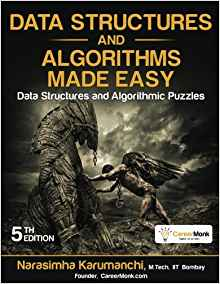
\includegraphics[height=6cm, width=5cm]{figs/fig_gerais/capa_livro_made_easy.jpeg}

\end{column}

\begin{column}{.5\textwidth}
\centering
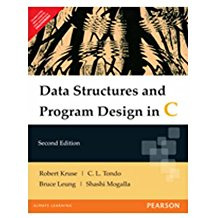
\includegraphics[height=6cm, width=5cm]{figs/fig_gerais/capa_livro_program_design_C.jpeg}

\end{column}

\end{columns}


\end{frame}
%-----------------------------------------------------------------------

\begin{frame}
\frametitle{Conteúdo programático}

   \textcolor{red}{Há um documento específico sobre isto $=$ Plano de Ensino}
    
\end{frame}


%-----------------------------------------------------------------------
\begin{frame}
\frametitle{Bibliografia UDESC}

    \textcolor{red}{Há um documento específico sobre isto $=$ Plano de Ensino}
      
 \end{frame}

%-----------------------------------------------

\begin{frame}
\frametitle{Conteúdo programático}

 \textcolor{red}{Há um documento específico sobre isto $=$ Plano de Ensino}

\end{frame}
---------------------------

\subsection{Ferramentas}
\begin{frame}

    \frametitle{Ferramentas ... nesta ordem}

    \begin{itemize}
     \item Linux 
      \item Linguagem C (ora o compilador g++)
      \item Codeblock
      

      % \url{http://ccl.northwestern.edu/netlogo/docs/} (escondido in WEB)
      
    \end{itemize}
\end{frame}

%%%%%%%%%%%%%%%%%%%%%%%%%%%%%%%%%%%%%%%%%%%%%%%%%%%%%%%%%%%%%%%%%%%%%

\subsection{Metodologia e avaliação}  

\begin{frame}[allowframebreaks=0.9]

\frametitle{Metodologia e avaliação}

\textbf{Metodologia:} \\

\textit{As aulas serão expositivas e práticas. A cada novo assunto tratado,
 exemplos  são demonstrados utilizando ferramentas computacionais adequadas
  para consolidar os conceitos 
 tratados. 
 }


\newpage
    \textbf{Avaliação}

    \begin{itemize}
    \item Três provas -- $\approx$  90\%\\
      
	\quad \textcolor{red}{$\bullet$}~$P_1$: xx/ago\\
	\quad \textcolor{red}{$\bullet$}~$P_2$: xx/set\\
		\quad \textcolor{red}{$\bullet$}~$P_3$: xx/set\\
	\quad \textcolor{red}{$\bullet$}~$P_4$: yy/out\\
		\quad \textcolor{red}{$\bullet$}~$P_5$: yy/nov\\
	\quad \textcolor{red}{$\bullet$}~$P_F$: zz/nov\\(provão: todo conteúdo)

      \item Exercícios de laboratório  -- $\approx$ \%
       
      \item Presença e participação: 75\% é o mínimo obrigatório
      para a UDESC. Quem quiser faltar por razões diversas,
       ou assuntos específicos, trate pessoalmente com o professor.
        
      \item Tarefas extras que geram pontos por excelência 
      
      \item Média para aprovação: 6,0 (seis)\\
      Nota maior ou igual a 6,0, repito a mesma no Exame Final. 
      Caso contrário, regras da UDESC se aplicam.
      
%%%      \item Sitio para entrega de trabalhos: \textbf{\url{https://www.cloudwok.com/u/mnG8}}
      
      \item Sitio das avaliações: \textbf{\url{https://run.codes/Users/login}} 
      código da disciplina: \textbf{GEPZ}
      
    \end{itemize}

\end{frame}



\subsection{Dinâmica}
\begin{frame} [allowframebreaks=0.9]

    \frametitle{Dinâmica de Aula}

    \begin{itemize}
    
       \item Há um monitor na disciplina -- Lucas -- ver no site de monitoria da UDESC 
       os horários
       
       \item Há uma lista de discussão (para avisos e dúvidas gerais):  \textbf{\url{eda-lista@googlegroups.com}}
       
      \item $\approx $ Teoria na 3a. feira
      \item $\approx $Prática na 5a. feira
      \item E/ou 50\% do tempo em teoria, 50\% implementações 
      \item Onde tudo vai estar atualizado?
   \end{itemize}
    \pause
 
 \newpage
    
  \begin{itemize}    
      \item \textcolor{red}{\textbf{\url{https://github.com/claudiosa/CCS/tree/master/estrutura_dados_EDA}}} 
     
      \item Ou seja, tudo vai estar \textit{rolando} no GitHub do professor
      
      \item No Google: \texttt{github + claudiosa}
   
      \item Finalmente ...   
  \end{itemize}
    
    
    \pause
    \newpage
    
    \begin{itemize}    
    
   \item Questões específicas (leia-se: notas, dor-de-dente, etc) venha falar 
   pessoalmente com o professor!
      
   \end{itemize}

\end{frame}



%%%%%%%%%%%%%%%%%%%%%%%%%%%%%%%%%%%%%%%%%%%%%%%%%%%%%%%%%%%%%%%%%%%%%

\subsection{Referências}  
%[allowframebreaks=0.9]

%-------------------------------------
\begin{frame}[allowframebreaks=0.9]
\frametitle{Bibliografia}  

\textbf{Básica:} 
\begin{itemize}

\item   \textcolor{red}{Há um documento específico sobre isto $=$ Plano de Ensino} ... veja em detalhes
tudo que foi escrito aqui

\item Mais uma vez: \url{https://github.com/claudiosa/CCS/tree/master/estrutura_dados_EDA}

\end{itemize}
\end{frame}

%-------------------------------------------------------------------------------------------------
\begin{frame}[allowframebreaks=0.9]
\frametitle{Antes de Começarmos ....}  


\begin{itemize}

\item Todos os cursos de Estrutura de Dados começam com uma motivação em torno
 da área para Ciência   

\item Vou omitir ... mas reflita se ela é ou não onipresente no nosso cotidiano?

\item Exemplos: bancos eletronicos, web, smartphones, etc
\end{itemize}


\end{frame}
%-------------------------------------------------------------------------------------------------



%%%%%%%%%%%%%%%%%%%%%%%%%%%%%%%%%%%%%%%%%%%%%%%%%%%%%%%%%%%%%%%%%%%%%
